\documentclass[compress]{beamer}
\usepackage{ifthen,verbatim}

\newcommand{\isnote}{}
\xdefinecolor{lightyellow}{rgb}{1.,1.,0.25}
\xdefinecolor{darkblue}{rgb}{0.1,0.1,0.7}

%% Uncomment this to get annotations
%% \def\notes{\addtocounter{page}{-1}
%%            \renewcommand{\isnote}{*}
%% 	   \beamertemplateshadingbackground{lightyellow}{white}
%%            \begin{frame}
%%            \frametitle{Notes for the previous page (page \insertpagenumber)}
%%            \itemize}
%% \def\endnotes{\enditemize
%% 	      \end{frame}
%%               \beamertemplateshadingbackground{white}{white}
%%               \renewcommand{\isnote}{}}

%% Uncomment this to not get annotations
\def\notes{\comment}
\def\endnotes{\endcomment}

\setbeamertemplate{navigation symbols}{}
\setbeamertemplate{headline}{\mbox{ } \hfill
\begin{minipage}{5.5 cm}
\vspace{-0.75 cm} \small
\end{minipage} \hfill
\begin{minipage}{4.5 cm}
\vspace{-0.75 cm} \small
\begin{flushright}
\ifthenelse{\equal{\insertpagenumber}{1}}{}{Jim Pivarski \hspace{0.2 cm} \insertpagenumber\isnote/\pageref{numpages}}
\end{flushright}
\end{minipage}\mbox{\hspace{0.2 cm}}\includegraphics[height=1 cm]{../cmslogo} \hspace{0.1 cm} \includegraphics[height=1 cm]{../tamulogo} \hspace{0.01 cm} \vspace{-1.05 cm}}

\newcommand{\s}[1]{{\mbox{\scriptsize #1}}}

\begin{document}
\begin{frame}
\vfill
\begin{center}
\textcolor{darkblue}{\Large Current Alignment Systematics: \\ \vspace{0.2 cm} Consequences for $Z'$}

\vfill
\begin{columns}
\column{0.3\linewidth}
\begin{center}
\large
Jim Pivarski
\end{center}
\end{columns}

\begin{columns}
\column{0.3\linewidth}
\begin{center}
\scriptsize
{\it Texas A\&M University}
\end{center}
\end{columns}

\vfill
 6 August, 2010

\end{center}
\end{frame}

%% \begin{notes}
%% \item This is the annotated version of my talk.
%% \item If you want the version that I am presenting, download the one
%% labeled ``slides'' on Indico (or just ignore these yellow pages).
%% \item The annotated version is provided for extra detail and a written
%% record of comments that I intend to make orally.
%% \item Yellow notes refer to the content on the {\it previous} page.
%% \item All other slides are identical for the two versions.
%% \end{notes}

\small

\begin{frame}
\frametitle{Motivation}
\begin{itemize}
\item Motivation \#1: we want to know how much the HW-TB discrepancies we've been discussing actually matter for physics ($Z'$ will be the most affected analysis)
\item Motivation \#2: part of what we need to provide is a quantitiative estimate of our uncertainties for analyses to study systematics
\begin{itemize}
\item typical systematics study: physics result $y$ depends on an imperfectly known quantity $x$ as $y = f(x)$
\item experimenter varies $\Delta x = x_1 - x_2$ and observes change in $f(x_1) - f(x_2)$, but how much $\Delta x$ variation is appropriate?
\item in the barrel, we can now answer that: \mbox{$\Delta x = x_\s{HW} - x_\s{TB}$\hspace{-1 cm}}
\item in the endcap, Samir's disk-shift study quantifies $f(x)$, but we don't yet have a systematic study of $\Delta x$
\end{itemize}
\item Only studied leading discrepancies in each dimension:
\begin{itemize}
\item pure twist (0.5~mrad rotations around global $\vec{R}$), no individual-chamber differences
\item local-$y$ differences, chamber-by-chamber
\item Samir's disk-shift study quantifies current leading uncertainty in endcap
\end{itemize}
\end{itemize}
\end{frame}

\begin{frame}
\frametitle{Comment}
\begin{itemize}
\item This is not a statement about whether HW is more correct than TB or vice-versa
\begin{itemize}
\item it does not rely on a model of why either one of them might be biased
\item it relies on the shape and magnitude of the empirically observed differences
\end{itemize}
\item We assume that we don't know which is correct, so we are
potentially making an error the size of the difference between them: that's the uncertainty
\end{itemize}
\end{frame}

\begin{frame}
\frametitle{Tested geometries: 1.\ twist}
\begin{itemize}
\item Systematic trends only, no individual-chamber differences (systematic trends are bigger than the individual differences)
\begin{itemize}
\item all chambers rotated 0.5~mrad in $\phi_z$ and translated in local-$x$ to line up, just as we see in the residuals plots
\item same slope in all stations, just as we see in the residuals plots
\end{itemize}
\end{itemize}

\includegraphics[width=0.49\linewidth]{twist_station1.pdf}
\includegraphics[width=0.49\linewidth]{twist_station2.pdf}

\includegraphics[width=0.49\linewidth]{twist_station3.pdf}
\includegraphics[width=0.49\linewidth]{twist_station4.pdf}
\end{frame}

\begin{frame}
\frametitle{Quantities of interest for tracks}
\begin{columns}
\column{0.6\linewidth}
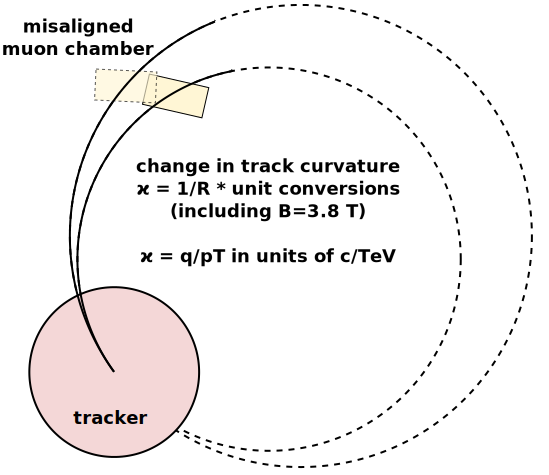
\includegraphics[width=\linewidth]{units.png}
\column{0.4\linewidth}
\begin{itemize}
\item In principle, misalignment can affect all five track parameters
\item But we're only interested in curvature errors for
from twist and $\eta$ errors from local-$y$
\item Express curvature as $\kappa = q/p_T$, errors as
$\kappa_\s{refit} - \kappa_\s{gen}$
\item Better than $pT_\s{refit} - pT_\s{gen}$ because of the simple
relationship between $\kappa$ and residuals: $\Delta \kappa$ is more Gaussian
\end{itemize}
\end{columns}
\end{frame}

\begin{frame}
\frametitle{Effect of twist}
\begin{itemize}
\item Regular pattern within the barrel: error in $\kappa$ is $(0.16\mbox{ $c$/TeV}) \times \eta$
\item $\eta > 1$ region is the barrel-endcap overlap: complicated in
this study because only the barrel was twisted (not something that
could happen with TB constants)
\item Bias is comparable to resolution: resolving twist is important
\end{itemize}

\begin{columns}
\column{0.5\linewidth}
\begin{center}
Ideal
\end{center}
\includegraphics[height=\linewidth, angle=90]{curvbias_vseta_ideal_1100_GlobalMuons2.pdf}

\column{0.5\linewidth}
\begin{center}
0.5~mrad twist
\end{center}
\includegraphics[height=\linewidth, angle=90]{curvbias_vseta_twist0_5mrad_1100_GlobalMuons2.pdf}
\end{columns}
\end{frame}

\begin{frame}
\frametitle{Effect of twist: more tests}

\begin{columns}
\column{0.5\linewidth}
Increases with track momentum (e.g.\ from higher-mass $Z'$s)

\includegraphics[height=\linewidth, angle=90]{curvbias_vseta_twist0_5mrad_1100_GlobalMuons2.pdf}

\includegraphics[height=\linewidth, angle=90]{curvbias_vseta_twist0_5mrad_2000_GlobalMuons2.pdf}

\column{0.5\linewidth}
Reverses when twist is reversed

\includegraphics[height=\linewidth, angle=90]{curvbias_vseta_twist0_5mrad_1100_GlobalMuons2.pdf}

\includegraphics[height=\linewidth, angle=90]{curvbias_vseta_antitwist0_5mrad_1100_GlobalMuons2.pdf}
\end{columns}
\end{frame}

\begin{frame}
\frametitle{Effect of twist: more tests}
\begin{itemize}
\item There are multiple refitting algorithms for reconstructing
TeV-muons to try to solve the problem of muon-showering
\item Misalignment effect doesn't depend strongly on algorithm
\end{itemize}

\vfill
\begin{columns}
\column{0.33\linewidth}
\begin{center}
GlobalMuons
\end{center}
\includegraphics[height=\linewidth, angle=90]{curvbias_vseta_twist0_5mrad_1100_GlobalMuons2.pdf}

\column{0.33\linewidth}
\begin{center}
Picky
\end{center}
\includegraphics[height=\linewidth, angle=90]{curvbias_vseta_twist0_5mrad_1100_TeVMuons2picky.pdf}

\column{0.33\linewidth}
\begin{center}
FirstStation
\end{center}
\includegraphics[height=\linewidth, angle=90]{curvbias_vseta_twist0_5mrad_1100_TeVMuons2firstHit.pdf}
\end{columns}
\end{frame}

\begin{frame}
\frametitle{Effect of twist: versus $p_T$}
\begin{itemize}
\item Since the effect also depends on $p_T$ (high-momentum tracks rely on muon chambers more, and get more biased), look at bias in an extreme $0.9 < \eta < 1.0$ slice
\item This would be done better with a muon-gun with a uniform distribution in $p_T$
\end{itemize}

\vfill
\begin{columns}
\column{0.5\linewidth}
\begin{center}
Ideal
\end{center}
\includegraphics[height=\linewidth, angle=90]{curvbias_vspt_ideal_GlobalMuons2.pdf}

\column{0.5\linewidth}
\begin{center}
0.5~mrad twist
\end{center}
\includegraphics[height=\linewidth, angle=90]{curvbias_vspt_twist0_5mrad_GlobalMuons2.pdf}
\end{columns}
\end{frame}

\begin{frame}
\frametitle{Effect of twist: summary}
\begin{itemize}
\item Both dependencies on one plot; color scale is average $\Delta\kappa$ in $c$/TeV (we get to see the bias, but not the width of the distribution)
\item Bilinear fit to the 2-D distribution: $\Delta\kappa \approx (0.12\mbox{ $c$/TeV})\eta + (0.1)\eta p_T$
\end{itemize}
\begin{center}
\includegraphics[height=0.9\linewidth, angle=90]{trackdistort2d_twist0_5mrad_GlobalMuons2.pdf}
\end{center}
\label{page:summary}
\end{frame}

\begin{frame}
\frametitle{Tested geometries: 2.\ local-$y$}
\begin{itemize}
\item The HW$-$TB differences that Aysen sent by HyperNews
\item Only local-$y$, no other directions
\end{itemize}

\vfill
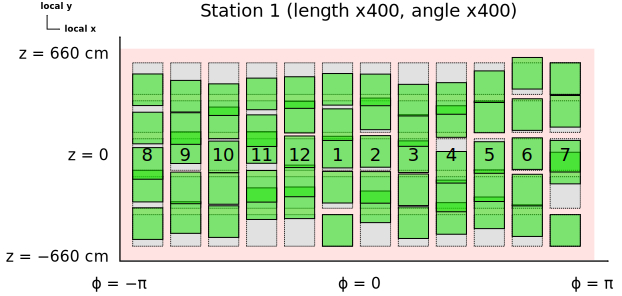
\includegraphics[width=0.49\linewidth]{localy_station1.pdf}
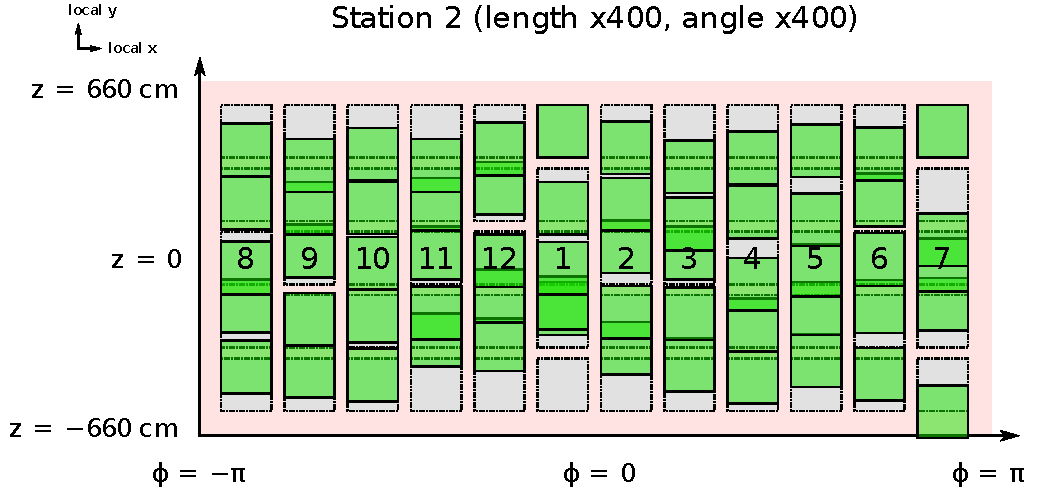
\includegraphics[width=0.49\linewidth]{localy_station2.pdf}

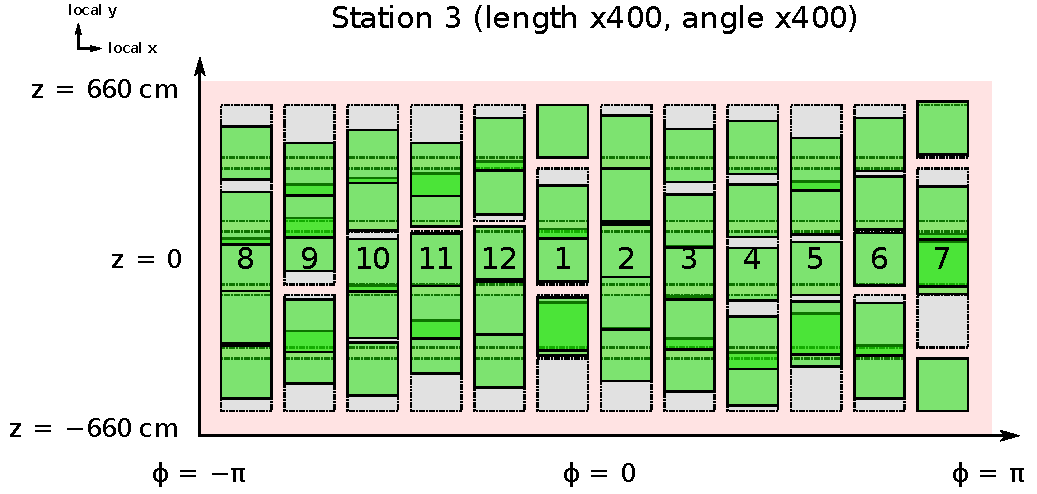
\includegraphics[width=0.49\linewidth]{localy_station3.pdf}
\includegraphics[width=0.49\linewidth]{localy_station4.pdf}
\end{frame}

\begin{frame}
\frametitle{Effect of local-$y$}
\begin{itemize}
\item Left: $\eta_\s{refit} - \eta_\s{gen}$ color scale versus $\eta$ and $\phi$ (you can see the individual chambers, even though high $\eta$ tracks pass through different wheels
\item Right: 1D $\eta_\s{refit} - \eta_\s{gen}$ distribution with and without misalignment; biases are comparable to the resolution
\end{itemize}

\vfill
\includegraphics[height=0.59\linewidth, angle=90]{etadistort_GlobalMuons2.pdf}
\includegraphics[height=0.39\linewidth, angle=90]{eta1d_GlobalMuons2.pdf}
\end{frame}

\begin{frame}
\frametitle{Effect of local-$y$}
\begin{itemize}
\item Different reconstruction method: FirstStation instead of GlobalMuon, only sensitive to station~1
\item Track-fits no longer mix different wheels
\item Less of an impact on $\Delta\eta$
\end{itemize}

\vfill
\includegraphics[height=0.59\linewidth, angle=90]{etadistort_TeVMuons2firstHit.pdf}
\includegraphics[height=0.39\linewidth, angle=90]{eta1d_TeVMuons2firstHit.pdf}
\end{frame}

\begin{frame}
\frametitle{Effect on $Z'$ mass}
\begin{itemize}
\item Want to quantify fractional error in mass: $(m_\s{refit} - m_\s{gen})/m_\s{gen}$
\item Complicated by the fact that $Z'$ has two daughters, sampling different parts of the detector
\item Key variable 1: $\eta_\s{lead} - \eta_\s{sublead}$ where the leading muon is the one with the highest $p_T$
\item Key variable 2: $q_\s{lead}$ ($\Delta\kappa$ that {\it raises} $\mu^+$ $p_T$ must {\it lower} $\mu^-$ $p_T$)
\item Shape far from $\eta_\s{lead} - \eta_\s{sublead} = 0$ depends on clipping (next slide)
\end{itemize}

\vfill
\includegraphics[height=0.49\linewidth, angle=90]{massbias_ideal_1100_GlobalMuons2_plus.pdf}
\includegraphics[height=0.49\linewidth, angle=90]{massbias_twist0_5mrad_1100_GlobalMuons2_plus.pdf}
\end{frame}

\begin{frame}
\frametitle{Effect on $Z'$ mass: aside}
\vspace{0.5 cm}
\includegraphics[height=0.49\linewidth, angle=90]{massbias_twist0_5mrad_1100_GlobalMuons2_plus.pdf}
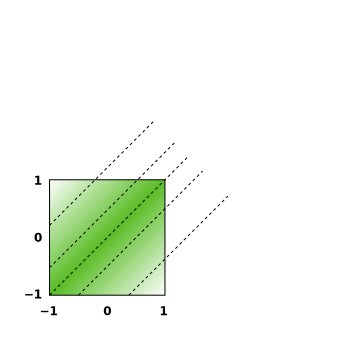
\includegraphics[width=0.49\linewidth]{clipping.png}

\vspace{-8.3 cm}
\begin{itemize}
\item To see only the effect of barrel twist on this plot, we must impose $|\eta| < 1.0$ for both daughters
\item This confines the daughters to a sqaure region in $\eta_1$-$\eta_2$ (always the case for a $Z'$ analysis, but usually $|\eta| < 2.4$)
\item The slope of $(m_\s{refit} - m_\s{gen})/m_\s{gen}$ \\ near $\eta_1 - \eta_2 = 0$ is due to misalignment; \\ the slope at high $|\eta_1 - \eta_2|$ is influenced \\ by clipping
\end{itemize}
\end{frame}

\begin{frame}
\frametitle{Effect on $Z'$ mass: more tests}
\begin{columns}
\column{0.5\linewidth}
Direction flips when we look at leading muon = $\mu^-$

\vspace{0.2 cm}
\includegraphics[height=0.95\linewidth, angle=90]{massbias_twist0_5mrad_1100_GlobalMuons2_plus.pdf}

\includegraphics[height=0.95\linewidth, angle=90]{massbias_twist0_5mrad_1100_GlobalMuons2_minus.pdf}

\column{0.5\linewidth}
Direction flips when we reverse twist

\vspace{0.2 cm}
\includegraphics[height=0.95\linewidth, angle=90]{massbias_twist0_5mrad_1100_GlobalMuons2_plus.pdf}

\includegraphics[height=0.95\linewidth, angle=90]{massbias_antitwist0_5mrad_1100_GlobalMuons2_plus.pdf}
\end{columns}
\end{frame}

\begin{frame}
\frametitle{Effect on $Z'$ mass: bottom line}
\begin{itemize}
\item Now showing $(m_\s{refit} - m_\s{gen})/m_\s{gen}$ in profile to
see how error from misalignment compares with intrinsic resolution
\item Local-$y$ errors (\textcolor{red}{red}) are never an issue: mass
resolution is dominated by $p_T$ uncertainties
\item Twist (\textcolor{blue}{blue}) broadens 4.3\% barrel resolution $\to$ 5.8\% for an energy-frontier $Z'$ (1100~GeV/$c^2$)--- 50--100~pb$^{-1}$ analyses

Smeared peak is about $\sqrt{2}$ times lower than ideal peak: would
require twice the data for a discovery

\item Becomes worse for higher masses
\end{itemize}

\includegraphics[height=0.32\linewidth, angle=90]{massdistribution_1100_GlobalMuons2.pdf}
\includegraphics[height=0.32\linewidth, angle=90]{massdistribution_2000_GlobalMuons2.pdf}
\includegraphics[height=0.32\linewidth, angle=90]{massdistribution_3000_GlobalMuons2.pdf}
\end{frame}

%% \begin{frame}
%% \frametitle{Outline}
%% \begin{itemize}\setlength{\itemsep}{0.75 cm}
%% \item 
%% \end{itemize}
%% %% \hspace{-0.83 cm} \textcolor{darkblue}{\Large Outline2}
%% \end{frame}

%% \section*{First section}
%% \begin{frame}
%% \begin{center}
%% \Huge \textcolor{blue}{First section}
%% \end{center}
%% \end{frame}

\begin{frame}
\frametitle{Conclusions}
\begin{itemize}
\item The HW-TB comparisons in the barrel quantify the leading
systematic uncertainties in chamber positions; this study relates them
to muon momentum and $Z'$ mass bias
\item The twist and the local-$y$ differences that we have been
discussing both lead to noticible biases in physics quantities
(comparable in size to the resolution for an ideal detector)
\item But only the twist leads to noticible biases in $Z'$ mass (and hence could delay discovery due to a less-significant peak)
\end{itemize}

\vfill
\hspace{-0.83 cm} \textcolor{darkblue}{\Large Post-conclusion}

\scriptsize

\vspace{0.1 cm}
\begin{itemize}
\item Curvature bias in fully-fitted tracks provides a way to test for twist with existant data: $\Delta\kappa$ from split-cosmics should be $\Delta\kappa = (0.12\mbox{ $c$/TeV} + 0.1 p_T) \cot\theta$ for a twisted geometry (from page~\pageref{page:summary}), where $\theta$ is the angle with respect to horizon
\item Different technique from TB alignment: fully-fitted tracks, checking for agreement between top and bottom halves, rather than tracker-vs-muon system
\item Do we have enough 200~GeV/$c$ tracks at $\cot\theta \approx 1$ to see a 0.13~$c$/TeV difference in curvature?  No, the whole CRAFT-08 sample (without splitting by $\cot\theta$) had only sensitivity to 0.6~$c$/TeV.  But maybe Jordan applied cuts that can be loosened?
\end{itemize}
\label{numpages}
\end{frame}

\end{document}
